\section{Topic}
\label{sec:topic}



\subsection{Notation}
Throughout this Chapter the following notation is used:
\begin{itemize}
    \item $ \phi $ is a conjunction of DL constraints.
    It is being checked for SAT.
    \item $ x - y \prec c $ is a general form
    of a DL constraint in $ \phi $ where $ \prec \; \in \{ <, \leq \} $.
    \item $ \mathbb{D} $ is a domain over which
    the variables and constants in $ \phi $ are defined
    (\eg $ \mathbb{R} $).
\end{itemize}



\subsection{Constraint Graph}
\begin{figure}[htb]
    \begin{center}
        \begin{tabular}{cc}
            \begin{minipage}{0.45\linewidth}
                \begin{center}
                    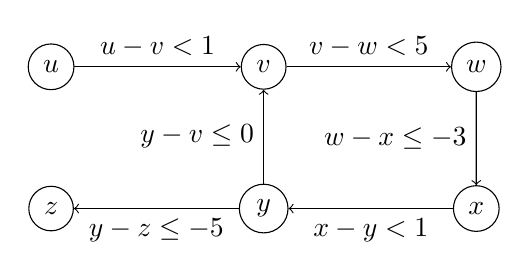
\begin{tikzpicture}[scale=0.9,state/.style={draw, circle, fill=none,text centered, text=black}]
    \node[state] (u) at (0, 2) {$u$};
    \node[state] (v) at (3, 2) {$v$};
    \node[state] (w) at (6, 2) {$w$};
    \node[state] (x) at (6, 0) {$x$};
    \node[state] (y) at (3, 0) {$y$};
    \node[state] (z) at (0, 0) {$z$};
    \draw [->] (u) -- node[anchor=south] {$ u-v < 1 $} (v);
    \draw [->] (v) -- node[anchor=south] {$ v-w < 5 $} (w);
    \draw [->] (w) -- node[anchor=east] {$ w-x \leq -3 $} (x);
    \draw [->] (x) -- node[anchor=north] {$ x-y < 1 $} (y);
    \draw [->] (y) -- node[anchor=north] {$ y-z \leq -5 $} (z);
    \draw [->] (y) -- node[anchor=east] {$ y-v \leq 0 $} (v);
\end{tikzpicture}

                \end{center}
            \end{minipage}
            &
            \begin{minipage}{0.45\linewidth}
                \begin{center}
                    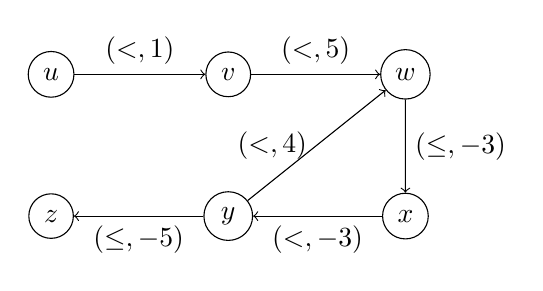
\begin{tikzpicture}[scale=0.9,state/.style={draw, circle, fill=none,text centered, text=black}]
    \node[state] (u) at (0, 2) {$u$};
    \node[state] (v) at (2.5, 2) {$v$};
    \node[state] (w) at (5, 2) {$w$};
    \node[state] (x) at (5, 0) {$x$};
    \node[state] (y) at (2.5, 0) {$y$};
    \node[state] (z) at (0, 0) {$z$};
    \draw [->] (u) -- node[anchor=south] {$ (<,1) $} (v);
    \draw [->] (v) -- node[anchor=south] {$ (<,5) $} (w);
    \draw [->] (w) -- node[anchor=west] {$ (\leq,-3) $} (x);
    \draw [->] (x) -- node[anchor=north] {$ (<,-3) $} (y);
    \draw [->] (y) -- node[anchor=north] {$ (\leq,-5) $} (z);
    \draw [->] (y) -- node[anchor=east] {$ (<,4) $} (w);
\end{tikzpicture}

                \end{center}
            \end{minipage}
        \end{tabular}
    \end{center}
    \caption{Examples of constraint graphs for
        Equation~\ref{eq:example-2} (left) and
        Equation~\ref{eq:example-3} (right).}
    \label{fig:contraints-graphs}
\end{figure}
Constraint graph (Figure~\ref{fig:contraints-graphs})
is a weighted directed graph which represents $ \phi $
and which is used by a DL constraints checker
(Figure~\ref{fig:lazy-and-incremental-approaches}) to test
if $ \phi $ is SAT.
In~\cite{cotton2004some} it is defined as follows:
\begin{definition}[Constraint Graph]
    \label{def:constraint-graph}
    The constraint graph is a graph $ \Gamma = (V,E,weight,op) $ where:
    \begin{itemize}
        \item $ V $ is a set of vertices. Each vertex $ x \in V $
        corresponds to one numeric variable occurring in $ x - y \prec c $.
        \item $ E $ is a set of directed edges. Each edge
        $ (x,y) \in E $ corresponds to $ x - y \prec c $.
        \item $ weight(x,y): E \mapsto \mathbb{D} $ is a weight function.
        It maps each edge $ (x,y) \in E $ to the constant
        $ c \in \mathbb{D} $ from the corresponding DL inequality
        $ x - y \prec c $.
        \item $ op(x,y): E \mapsto \{ <, \leq \} $ is a function which
        maps each edge $ (x,y) \in E $ to the operation
        $ \prec $ from the corresponding DL inequality
        $ x - y \prec c $.
    \end{itemize}
\end{definition}




\subsection{Negative Cycles in Constraint Graph}
There is a direct correspondence between a negative cycle
in a constraint graph and SAT of $ \phi $ represented by this graph.

A path in the graph corresponds to a sum of the corresponding
constraints. \Eg the path
$ u \rightarrow v \rightarrow w \rightarrow x $
in the left graph on Figure~\ref{fig:contraints-graphs}
corresponds to the following sum of the DL inequalities:
\begin{equation}
    \begin{aligned}
        u - v & < \;\;\; 1 \\
        v - w & < \;\;\; 5 \\
        w - x & \leq -3 \\
        \hline
        u - x & < \;\;\; 3
    \end{aligned}
\end{equation}
If at least one strict inequality is present
then the resulting inequality will also be strict.
This summation along a path can also be expressed with
an inferred transitivity constraint
(\eg~Equation~\ref{eq:transitivity-example}).
The transitivity constraint naturally follows from $ \phi $ and
therefore must be satisfied in order to satisfy $ \phi $.

A cycle in the constraint graph corresponds to an inequality
$ 0 \prec c $
which may cause a conflict in the following situations:
\begin{itemize}
    \item $ c < 0$
    \item $ c = 0 $ and $ \prec $ is $ < $
    (can be checked with $ op $ from Definition~\ref{def:constraint-graph})
\end{itemize}

An example of a conflict can be seen on the right graph
on Figure~\ref{fig:contraints-graphs}.
The conflict corresponds to the negative cycle
$ x \rightarrow y \rightarrow w \rightarrow x $
which corresponds to the following conflicting inequalities:
\begin{equation}
    \begin{aligned}
        x - y & < -3 \\
        y - w & < \;\;\; 4 \\
        w - x & \leq -3 \\
        \hline
        0 & < -2
    \end{aligned}
\end{equation}



\subsection{Bellman-Ford Algorithm for Constraint Graph}
\cite{cotton2004some} uses a Goldberg-Radzik~\cite{goldberg1993heuristic}
variant of the Bellman-Ford algorithm~\cite[p.651]{cormen2009introduction}
to detect negative cycles
and thus check $ \phi $ for SAT
(Algorithm~\ref{alg:goldberg-radzik}).
\cite{goldberg1993heuristic}~states that the algorithm has the same
worst-case complexity $ O(|V| \cdot |E|) $
as Bellman-Ford algorithm but is superior in practice.
Terminology and notation used in the algorithm are given below.
\begin{definition}[Source Vertex]
    The source vertex $ s \in V $ is a vertex from which
    the shortest paths to other vertices are computed.
\end{definition}
\begin{definition}[Shortest Path Weight]
    The shortest path weight~\cite[p.643]{cormen2009introduction}
    $ \delta(v) $ from the source vertex
    to $ v \in V $ is defined as the minimal sum of the weights of the edges
    of a path from the source vertex to $ v $ across all such paths
    (if at least one exist).
    If there is no path from the source vertex to $ v $
    then $ \delta(v) = \infty $.
    If there is a negative cycle on a path from the source vertex to $ v $
    then $ \delta(v) = -\infty $.
\end{definition}
\begin{definition}[Distance Estimating Function~\cite{cotton2004some}]
    The distance estimating function $ d(v): V \mapsto \mathbb{D} $
    is function which returns an upper bound on the distance
    from the source vertex to the given vertex $ v \in V $.
\end{definition}
\begin{definition}[Reduced Cost Function~\cite{goldberg1993heuristic}]
    The reduced cost function
    $ r_d(x,y): V \mapsto \mathbb{D} $ is
    defined as follows:
    $ r_d(x,y) = weight(x,y) + d(x) - d(y) $.
\end{definition}
\begin{definition}[Vertex Status]
    The vertex status
    $ status(x) = \{ unreached, labeled, scanned \} $
    is a function on vertices which shows a current state of
    a vertex $ x \in V $.
    $ status(x) = unreached $ means $ x $ has not been explored yet.
    $ status(x) = labeled $ means $ x $ has been explored \ie
    the distance estimate for it has been updated at least once
    and potentially it can be used to improve distance estimates to
    other vertices.
    $ status(x) = scanned $ means $ x $ has been completely explored
    and will not be considered further for improving distance estimates.
\end{definition}
\begin{definition}[Admissible Edge]
    Edge $ (x,y) \in E $ is called admissible if $ r_d(x,y) \leq 0 $.
\end{definition}
\begin{definition}[Admissible Graph]
    Admissible graph $ \Gamma_d $ is a subgraph
    of $ \Gamma $ composed of the admissible edges of $ \Gamma $.
\end{definition}

In Algorithm~\ref{alg:goldberg-radzik} distance estimates are iteratively
updated.
In~\cite[p.648]{cormen2009introduction} this process
is called "iterative edge relaxation".
It can also be seen as a series of different distance
estimate functions $ (d_0, d_1, d_2, d_3, \dots) $.
Each $ d_i $ in this series describes which distance estimates
have the vertices at some iteration of
the Algorithm~\ref{alg:goldberg-radzik}.

The idea of the Algorithm~\ref{alg:goldberg-radzik} is to use
the dynamically changing graph $ \Gamma_d $
(it changes whenever $ d $ changes)
to detect negative or zero cycles in the original graph $ \Gamma $.
The following theorem from~\cite{cotton2004some}
expresses this idea more formally.
\begin{theorem}
    \label{the:neg-cycle-in-cg}
    Given a constraint graph $ \Gamma $ and a series of distance estimating
    functions $ (d_0, d_1, d_2, d_3, \dots) $, $ \Gamma $ has a negative
    or zero cycle if and only if $ \Gamma_d $ has a cycle under some
    distance estimate $ d_k $.
    \begin{proof}
        $ \Rightarrow $ Case 1. $ \Gamma $ has a negative cycle
        $ N = (x_0, x_1, \dots, x_{n-1}, x_n) $ with $ x_n = x_0 $.
        To prove:
        $ \Gamma_d $ also has this cycle.
        In~\cite[pp.672-673]{cormen2009introduction} it
        is proven that if a graph has a negative cycle,
        then the distance estimation process $ (d_0, d_1, d_2, d_3, \dots) $
        will never converge.
        Therefore, for sufficiently large $ k $ there always will be some
        edge from $ N $ which can further update current $ d_k $ \ie
        $ \exists i, 0 \leq i < n: d_k(x_i) + weight(x_i, w_{i+1}) < d_k(x_{i+1}) $.

        It can be the case that at some further iteration a
        path $ p = s \rightarrow x_{i+1} $
        from the source vertex $ s $ to $ x_{i+1} $
        will be discovered and this path may give even better improvement
        than the mentioned one for $ d_k $
        \ie $ len(p) < d_k(x_i) + weight(x_i, w_{i+1}) $
        where $ len(p) $ is the length of the path $ p $.
        In this situation an edge from the path $ p $
        will be applied to update $ d $ and therefore
        edge $ (x_i, x_{i+1}) $
        will be excluded from $ \Gamma_d $
        because in this case
        $ r_d(x_i,x_{i+1}) = weight(x_i,x_{i+1}) + d_m(x_i) - d_m(x_{i+1}) = weight(x_i,x_{i+1}) + d_k(x_i) - len(p) > 0 $
        where $ m > k $ is some further iteration in which
        the path $ p $ has been used to update distance estimate
        to the vertex $ x_{i+1} $, \ie $ d_m(x_{i+1}) = len(p) $,
        and the distance estimate to the
        vertex $ x_i $ has not been updated, \ie $ d_m(x_i) = d_k(x_i) $.
        A simple example is given
        on~Figure~\ref{fig:negative-cycles-in-graphs} on the left
        where in the very beginning a path $ (s,x) $
        from $ s $ to $ x $
        will be the shortest known path until the negative edge
        $ (w,x) $ is discovered and the path $ (s,v,w,x) $
        will be shorter.

        Since a graph has a finite number of edges, the number of such
        paths, which connect $ s $ and a vertex in $ N $, is also finite.
        Therefore \WLOG we can assume that
        the $ k $ is sufficiently large and
        all this paths have already been discovered and applied
        to improve $ d $.
        If these paths are not contained in other negative cycles,
        they cannot be used in further iterations
        (see "convergence property" and "path relaxation property"
        in~\cite[p.650]{cormen2009introduction}).

        Suppose, however, that there is another negative cycle which
        has a connection with $ N $.
        An example is given
        on~Figure~\ref{fig:negative-cycles-in-graphs} on the right
        where the negative cycle $ (u,v,w,z,u) $ has the common vertex
        $ w $ with another negative cycle $ (w,x,y,w) $.
        So this cycle can interfere with $ N $ and cause some of the
        edges of $ N $ to be excluded from $ \Gamma_d $ by providing
        a better update to the vertex $ x_{i+1} $ than the edge
        $ (x_i,x_{i+1}) $.
        However, in order to provide this update to $ x_{i+1} $
        algorithm needs to enter this cycle and complete it
        \ie follow all its edges and apply updates.
        Therefore, again, \WLOG we can regard this interfering
        negative cycle
        instead of $ N $.

        Thus, \WLOG let the regarded cycle $ N $ be a cycle
        which does not interfere with other cycles and
        let $ k $ be sufficiently large such that all paths, which
        connect $ s $ with vertices of $ N $
        and which are not contained in any negative cycles,
        have already been
        applied to improve $ d $ and therefore will not be applied
        in the further iterations.
        Then the edge $ (x_i,x_{i+1}) $ will trigger a series of updates
        of $ d $ which will be applied along $ N $.
        There will be no interference from other negative cycles.
        Otherwise we would regard them instead of $ N $.
        There will be no interference from paths,
        which start at $ s $ and end at some vertex of $ N $,
        because otherwise we would choose larger $ k $.
        Therefore after this series of updates, algorithm
        arrives at some estimate $ d_{k'}, k'>k $ for which
        the reduced cost function on the edges of $ N $ will be zero
        or less and therefore the edges of $ N $ will be in $ \Gamma_d $
        by definition.

        Case 2. $ \Gamma $ has no negative cycles but it has
        a zero weight cycle $ Z = (x_0, x_1, \dots, x_{n-1}, x_n) $
        with $ x5_n = x_0 $.
        Then ...
        \\

        $ \Leftarrow $ fff
    \end{proof}
\end{theorem}
~
\begin{figure}[htb]
    \begin{center}
        \begin{tabular}{cc}
            \begin{minipage}{0.45\linewidth}
                \begin{center}
                    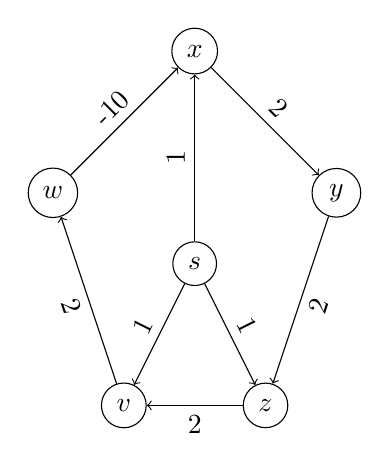
\begin{tikzpicture}[scale=0.9,state/.style={draw, circle, fill=none,text centered, text=black}]
    \node[state] (s) at (0, 0) {$s$};
    \node[state] (v) at (-1, -2) {$v$};
    \node[state] (w) at (-2, 1) {$w$};
    \node[state] (x) at (0, 3) {$x$};
    \node[state] (y) at (2, 1) {$y$};
    \node[state] (z) at (1, -2) {$z$};

    \draw [->] (s) -- node[anchor=south, sloped] {1} (v);
    \draw [->] (s) -- node[anchor=south, sloped] {1} (x);
    \draw [->] (s) -- node[anchor=south, sloped] {1} (z);

    \draw [->] (v) -- node[anchor=north, sloped] {2} (w);
    \draw [->] (w) -- node[anchor=south, sloped] {-10} (x);
    \draw [->] (x) -- node[anchor=south, sloped] {2} (y);
    \draw [->] (y) -- node[anchor=north, sloped] {2} (z);
    \draw [->] (z) -- node[anchor=north, sloped] {2} (v);
\end{tikzpicture}

                \end{center}
            \end{minipage}
            &
            \begin{minipage}{0.45\linewidth}
                \begin{center}
                    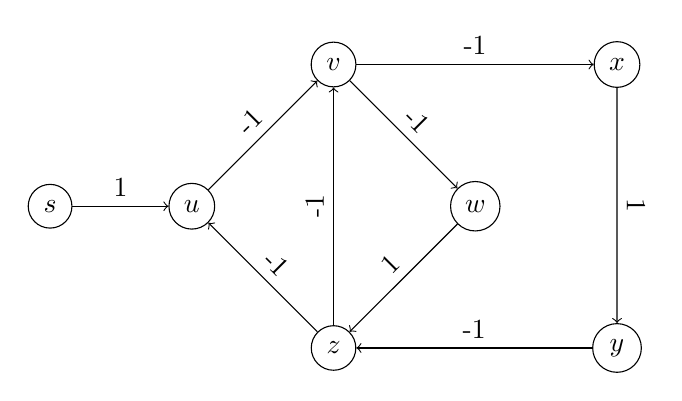
\begin{tikzpicture}[scale=0.9,state/.style={draw, circle, fill=none,text centered, text=black}]
    \node[state] (s) at (0, 0) {$s$};
    \node[state] (u) at (2, 0) {$u$};
    \node[state] (v) at (4, 2) {$v$};
    \node[state] (w) at (6, 0) {$w$};
    \node[state] (x) at (8, 2) {$x$};
    \node[state] (y) at (8, -2) {$y$};
    \node[state] (z) at (4, -2) {$z$};
    
    \draw [->] (s) -- node[anchor=south, sloped] {1} (u);
    \draw [->] (u) -- node[anchor=south, sloped] {-1} (v);
    \draw [->] (v) -- node[anchor=south, sloped] {-1} (w);
    \draw [->] (v) -- node[anchor=south, sloped] {-1} (x);
    \draw [->] (x) -- node[anchor=south, sloped] {1} (y);
    \draw [->] (y) -- node[anchor=south, sloped] {-1} (z);
    \draw [->] (w) -- node[anchor=south, sloped] {1} (z);
    \draw [->] (z) -- node[anchor=south, sloped] {-1} (u);
    \draw [->] (z) -- node[anchor=south, sloped] {-1} (v);
\end{tikzpicture}

                \end{center}
            \end{minipage}
        \end{tabular}
    \end{center}
    \caption{Example of negative cycles in graphs.}
    \label{fig:negative-cycles-in-graphs}
\end{figure}
~
\begin{Algorithm}
    \caption{An algorithm for checking if $ \phi $ which corresponds
        to the input constraint graph $ \Gamma = (V,E,weight,op) $ is SAT.
        It returns SAT or UNSAT status and a set of DL constraints
        corresponding to a conflict (in case of UNSAT).
        It is based on Bellman-Ford
        algorithm~\cite[p.561]{cormen2009introduction}.
        Goldberg-Radzik heuristic~\cite{goldberg1993heuristic},
        which is used here,
        suggests to scan a graph in a topological order.
        This algorithm uses
        depth first search~\cite[p.603]{cormen2009introduction} (DFS)
        and breadth first search~\cite[p.594]{cormen2009introduction} (BFS)
        for auxiliary tasks.}
    \label{alg:goldberg-radzik}
    \begin{algorithm}{Goldberg-Radzik}
        {\text{constraint graph} \Gamma = (V,E,weight,op),
            \text{source vertex} s \in V}
        \begin{FOR}{\mathrm{each \; vertex} \; x \in V}
            d(x) = \infty \\
            status(x) = unreached
        \end{FOR} \\
        d(s) = 0 \\
        status(s) = labeled \\
        A \= \varnothing \\
        B \= \{ s \} \\
        \begin{REPEAT} \\
            \begin{IF}{\Gamma_d \text{has a cycle} C \text{(DFS on} \Gamma_d \text{can be used to check it)}}
                l \= \text{length of} C \text{in} \Gamma \\
                \begin{IF}{l < 0}
                    \RETURN (UNSAT, \text{DL constraints corresponding to} L)
                \end{IF} \\
                \begin{IF}{\exists \; (x,y) \in L \text{such that} op(x,y) = \; <}
                    \RETURN (UNSAT, \text{DL constraints corresponding to} L)
                \end{IF}
            \end{IF} \\
            \begin{FOR}{\mathrm{each \; vertex} \; x \in B}
                \begin{IF}{x \text{has no outgoing admissible edges}}
                    B \= B \setminus \{ x \} \\
                    status(x) = scanned
                \end{IF}
            \end{FOR} \\
            A \= \text{set of unexplored vertices reachable from}
                    B \text{in} \Gamma_d
                    \text{(BFS on} \Gamma_d \text{can be used here)} \\
            A \= \text{sort} A \text{topologically using}
                    \Gamma_d \text{as an input graph}
                    \text{(DFS on} \Gamma_d \text{can be used here)} \\
            B \= \varnothing \\
            \begin{FOR}{\mathrm{each \; vertex} \; x \in A}
                status(x) = labeled \\
                \begin{FOR}{\mathrm{each \; edge} \; (x,y) \in E}
                    \begin{IF}{d(x) + weight(x,y) < d(y)}
                        d(y) \= d(x) + weight(x,y) \\
                        \begin{IF}{status(y) = unreached}
                            B \= B \cup \{ y \}
                        \end{IF} \\
                        status(y) \= labeled \\
                        status(x) \= scanned
                    \end{IF}
                \end{FOR}
            \end{FOR}
        \end{REPEAT} A \; is \; empty \\
        \RETURN (SAT, \varnothing) \\
    \end{algorithm}
\end{Algorithm}
Some notes to the Algorithm~\ref{alg:goldberg-radzik}:
\begin{itemize}
    \item In practice, checking $ \Gamma_d $ for a cycle (line~9) and
    computing a set of vertices reachable from $ B $ (line~15) can be
    done by only one DFS call.
    However, it is two logically distinct steps and therefore they
    are performed separately in the algorithm.
    \item Unexplored vertices (line~15) are vertices which have
    status $ unreached $ \ie they have not been processed yet at that
    particular step.
    \item If $ B $ is empty or no unexplored vertices
    are reachable from it (line~15) then $ A $ will be assigned an
    empty set.
\end{itemize}
